\documentclass[12pt]{article}
\usepackage{minted}
\usepackage{graphicx}
\usepackage{mathtools}
\usepackage{amsfonts}

\begin{document}
    \title{CS 559 Homework 1}
    \author{Stephen Szemis}
    \date{October 1, 2020}
    \maketitle

    I pledge my honor that I have abided by the Stevens honor system.

    \paragraph{Problem 1: Perceptron}
    \subparagraph{Part 1:}
    Yes. The NAND function can be linearly separable.
    \subparagraph{Part 2:}
    Let's run perception. We have to account for bias (not mentioned in slides) in
    order to actually converge here. All Points now will have an extra dimension 
    appended, this is just a 1 to help clean up the dot product. Example:
    \(P_1=(0, 1, 1)\) and \(P_1=(1, 1, 1)\). Our initial weights are then
    \(w=(1, 1, -\frac{1}{2})\) to account for our initial boundary.
    \begin{enumerate}
        \item 
        \(w_1^T=(1, 1, -\frac{1}{2}) \, P_1=(0, 1, 1) \) since 
        \((w_1 * P_1) > 0 \) that means
        \(P_1\) is classified as positive, which is wrong.
        So update \(w_2 = w_1 - P_1 = (1, 0, -\frac{3}{2})\)
        \item 
        \(w_2^T=(1, 0, -\frac{3}{2}) \, P_2=(1, 1, 1) \) since 
        \((w_2 * P_2) < 0 \) that means
        \(P_2\) is classified as negative, which is wrong.
        So update \(w_3 = w_2 + P_2 = (2, 1, -\frac{1}{2})\)
        \item 
        \(w_3^T=(2, 1, -\frac{1}{2}) \, P_3=(1, 0, 1) \) since 
        \((w_3 * P_3) > 0 \) that means
        \(P_3\) is classified as positive, which is wrong.
        So update \(w_4 = w_3 - P_3 = (1, 1, -\frac{3}{2})\)
        \item 
        \(w_4^T=(1, 1, -\frac{3}{2}) \, P_4=(0, 0, 1) \) since 
        \((w_4 * P_4) < 0 \) that means
        \(P_4\) is classified as negative, which is correct. No update.
        \item 
        \(w_5^T=(1, 1, -\frac{3}{2}) \, P_1=(0, 1, 1) \) since 
        \((w_5 * P_1) < 0 \) that means
        \(P_1\) is classified as negative, which is correct. No update.
        \item 
        \(w_6^T=(1, 1, -\frac{3}{2}) \, P_2=(1, 1, 1) \) since 
        \((w_6 * P_2) > 0 \) that means
        \(P_2\) is classified as positive, which is correct. No update.
        \item 
        \(w_7^T=(1, 1, -\frac{3}{2}) \, P_3=(1, 0, 1) \) since 
        \((w_7 * P_3) < 0 \) that means
        \(P_3\) is classified as negative, which is correct. No update.
    \end{enumerate}
    We've successfully classified all four points, so our weights and bias is
    correct. Our final decision boundary is \( x_1 + x_2 - \frac{3}{2} = 0 \).

    \paragraph{Problem 2: PCA and Eigenfaces}
    \subparagraph{Part 1: The code and eigenfaces}

    \inputminted{python}{Szemis_hw2.py}

    And here are the top ten eigenfaces.
    \begin{center}
    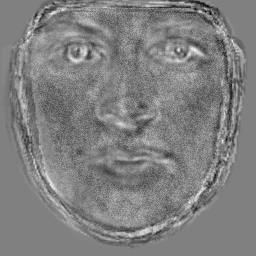
\includegraphics[width=5cm]{output_part1/eigenface_0.png}
    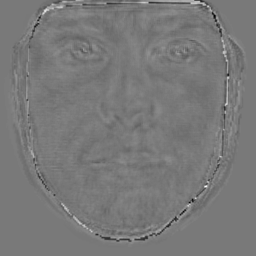
\includegraphics[width=5cm]{output_part1/eigenface_1.png}
    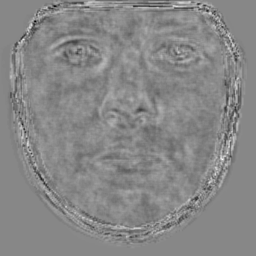
\includegraphics[width=5cm]{output_part1/eigenface_2.png}
    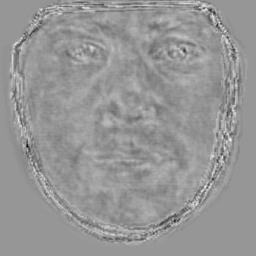
\includegraphics[width=5cm]{output_part1/eigenface_3.png}
    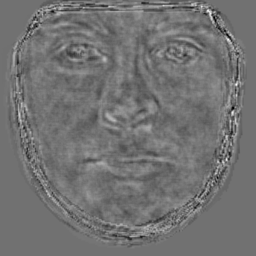
\includegraphics[width=5cm]{output_part1/eigenface_4.png}
    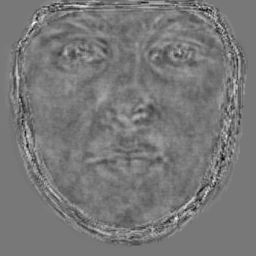
\includegraphics[width=5cm]{output_part1/eigenface_5.png}
    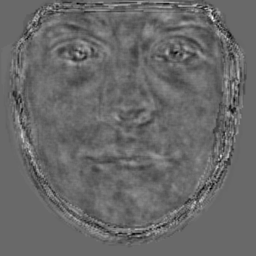
\includegraphics[width=5cm]{output_part1/eigenface_6.png}
    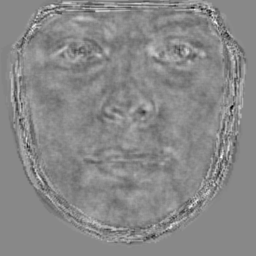
\includegraphics[width=5cm]{output_part1/eigenface_7.png}
    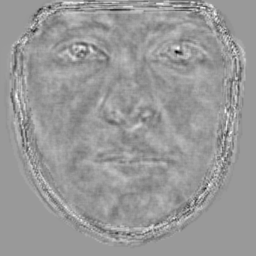
\includegraphics[width=5cm]{output_part1/eigenface_8.png}
    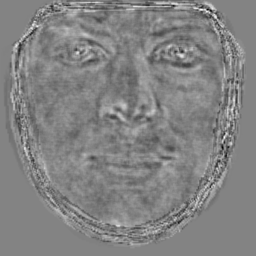
\includegraphics[width=5cm]{output_part1/eigenface_9.png}
    \end{center}
    
    \subparagraph{Part 2: Reconstruction}
    The necessary code is commented above.
    Here are the reconstructed images side by side with the originals.
    \begin{center}
    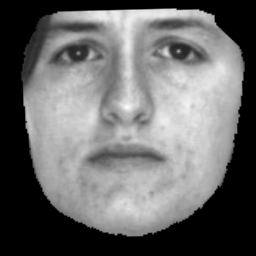
\includegraphics[width=5cm]{output_part2/original_0.png}
    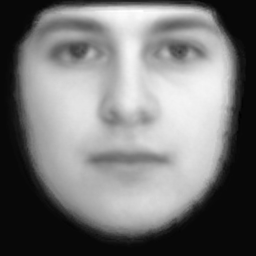
\includegraphics[width=5cm]{output_part2/reconstruct_0.png}
    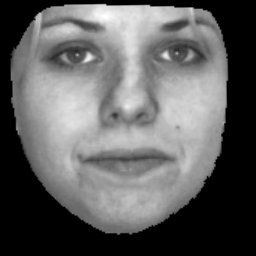
\includegraphics[width=5cm]{output_part2/original_1.png}
    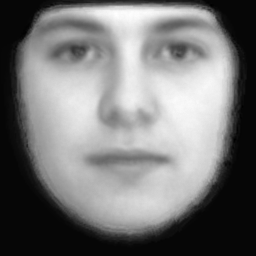
\includegraphics[width=5cm]{output_part2/reconstruct_1.png}
    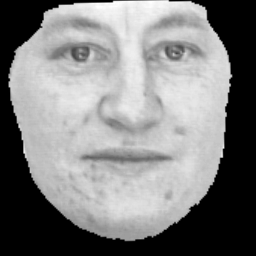
\includegraphics[width=5cm]{output_part2/original_2.png}
    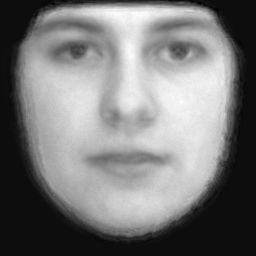
\includegraphics[width=5cm]{output_part2/reconstruct_2.png}
    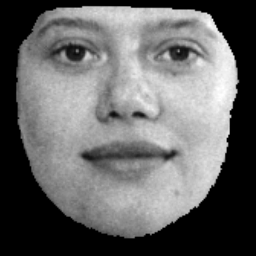
\includegraphics[width=5cm]{output_part2/original_3.png}
    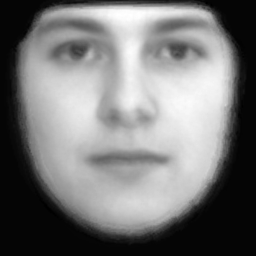
\includegraphics[width=5cm]{output_part2/reconstruct_3.png}
    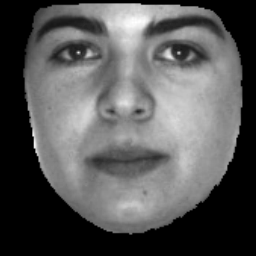
\includegraphics[width=5cm]{output_part2/original_4.png}
    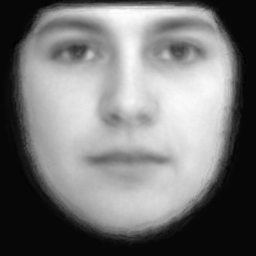
\includegraphics[width=5cm]{output_part2/reconstruct_4.png}
    \end{center}

    The reconstruction error was 16.81. I should note that we calculate the error
    per pixel, not just per image. So we end up dividing the normal error calculation by 256 * 256.

    \subparagraph{Part 3: Plotting K}
    As per usual, the comments will tell you which piece of code does what.
    Here is our graph of k increasing by 10, up to our max k value of 140.
    \begin{center}
    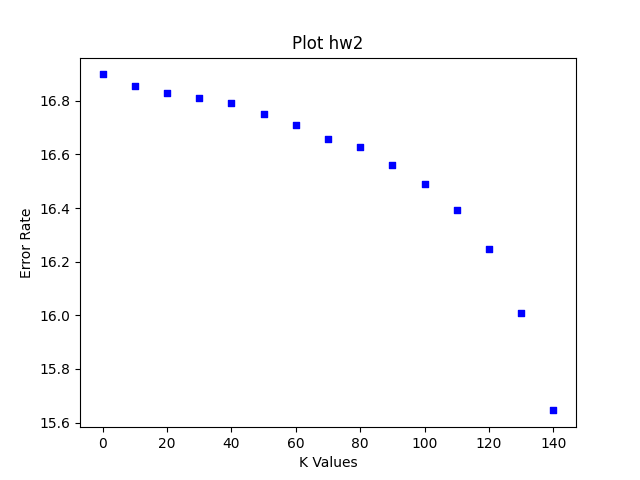
\includegraphics[width=10cm]{graph_part3.png}
    \end{center}
    It's clear to see that we get an exponential drop off in error as we increase k.
    This makes sense since as k approaches our original dimension D, we end up simply containing 
    all the information in our principal components. Of course, even at a large k, we still have a 
    massive decrease in dimensionality. And since our error is so low, it's easy to see that PCA and 
    eigenfaces are quiet effective at describing the necessary parts of the images.

\end{document}